\documentclass[11pt]{article}
\usepackage{graphicx}
\usepackage{float}
\usepackage[labelformat= empty]{caption}
\begin{document}
\include{epsf}
\thispagestyle{empty}
\title{{\LARGE\bf System Architecture Document}}
\author{{\Large\it Authors} \\
\vspace*{2.5in} 
\mbox{} \\
{\Large Title of Project}
\vspace*{2.5in} 
\mbox{} \\
\date{\today}
}
\maketitle

\tableofcontents

%\bibliographystyle{plain}
\newpage
\section{Introduction}
This introduction provides a brief overview of System Architecture Document for the current iteration of the Post Graduate Application Approval System. It consists of the purpose, scope, problem statement,project objectives, stakeholders and overview of the rest of the document.
\subsection{Purpose}
\paragraph{}This document provides the reader with an architectural overview of the Post Graduate Application Approval System. The primary purpose of this project is to create a single integrated system that facilitates application review and decision making.

\paragraph{}This document is intended to elucidate the major architectural decisions that have been made when designing and implementing the system. This is achieved by viewing the system architecture from various perspectives, called views. These views are intended to explain the system architecture through all levels of the development stack, from front-end to back-end.


\subsection{Scope}
The scope of this document is the design and implementation of the software based Post Graduate Application Approval System which consists of the application upload by the Post Graduate Officer, the intermediary application review by the Supervisor and the final application review made by the Post Graduate Coordinator.

\subsection{Problem Statement}
Currently, the School of EIE uses a paper based method for the approval of post graduate applications. The primary reasons for this, is as a result of academics not being trained on the SIMS system and paper trail to be kept for transparency purposes. This paper based system involves manual filling and can result in misplacement of documentation. Supervisors are contacted to review applications when the PGO physically sees them or sends an email. The turnaround time of approval of a PG application, the physical space manual filing takes up and the risk for misplacement of documents are all issues with the current process. In order to alleviate these issues a web based system will be used as a central repository for all applications to the School of EIE and manage the process of approval within the school.
\subsection{Project Objectives}
\subsection{Stakeholders}
The following lists the stakeholders in the development of this system.

\paragraph{School of Electrical and Information Engineering}
\begin{itemize}
	
	
	
	\item Mrs. Mumtaz Adam: The post graduate officer (PGO).
	
	\item Professor Ling Cheng: The post graduate coordinator (PGC).
	
	\item Supervisors: Various academics within the school who shall supervise applicants.
	
	\item The Applicant.
	
\end{itemize}

\paragraph{Development Team}
\begin{itemize}
	\item Professor Ekow Otoo: The product owner.
	
\end{itemize}
\subsection{Overview}
describe the structure and content of rest of report
\section{Architectural Goals and Constraints}
The architecture of the system has been designed to achieve the following objectives:
\begin{enumerate}
	\item To assist the application approval process by having all application documents and information in a single digital repository.
	\item To assist the Post Graduate Officer with the upload of application documents.
	\item To simplify application reviews by having a single integrated view of all important information for each decision maker.
	\item To prevent human error by providing notifications and weekly reminders about pending applications.
	
\end{enumerate}

The significant constraints kept in mind when developing the system were as follows:

\begin{enumerate}
	\item Security
	\item Ease of Use
	\item Paperless
\end{enumerate}
\section{Architectural Representation}
\subsection{Architectural Views}
The development of the system has various contributors each with their own priorities and tasks. As such, the system needs to be documented from various perspectives to aid, and eventually validate, the completion of a contributor's tasks. The system architecture shall be represented from the following views:

\begin{enumerate}
	\item Use Case View: This defines the high-level interactions between various actors and the system.
	\item Design View: This contains the class and architecture diagrams of the system.
	\item Process View: This displays the processes within the system that combine to perform the various interactions defined in the Use Case View.
	\item Component View: This displays the User Interface of the system.
	\item Database View: This contains the Entity-Relationship Diagram for the system database.
\end{enumerate} 
\subsection{Architectural Design Patterns}
ASP.NET Core framework was used in the implementation of the system. This follows the Model-View-Controller(MVC) design pattern. This design pattern separates the project into three distinct layers:

\begin{enumerate}
	\item Model: Defines the data structures of the system and directly handles all logic and data within the system. A model class communicates exclusively with its controller.
	\item View: A visual representation of a model. Typically in the form of a web page or a component of the web page. The view communicates exclusively with its controller.
	\item Controller: Accepts user input and maps it to instructions for models, views and potentially other controllers. Directly responsible for communication between components of the system.
	
	  
\end{enumerate} 

This framework and design pattern was chosen to enhance modularity of the system. This allows for: 
\begin{itemize}
	\item Parallel development
	\item Efficient code reuse
	\item Faster bug detection and tracking.
	\item Greater unit testing coverage.
	
\end{itemize} 
 
\subsection{Architectural Process}
what process was used to design the system.
\section{Architectural View Decomposition}
\subsection{Use-Case View}
use case diagram plus short description of each use case.
\subsubsection{Architecturally Significant Use Cases}
describe in detail the use cases that use the most critical part of the system (possibly fully dressed use cases for this)
\subsection{Design View}
\begin{figure}[H]
	\frame{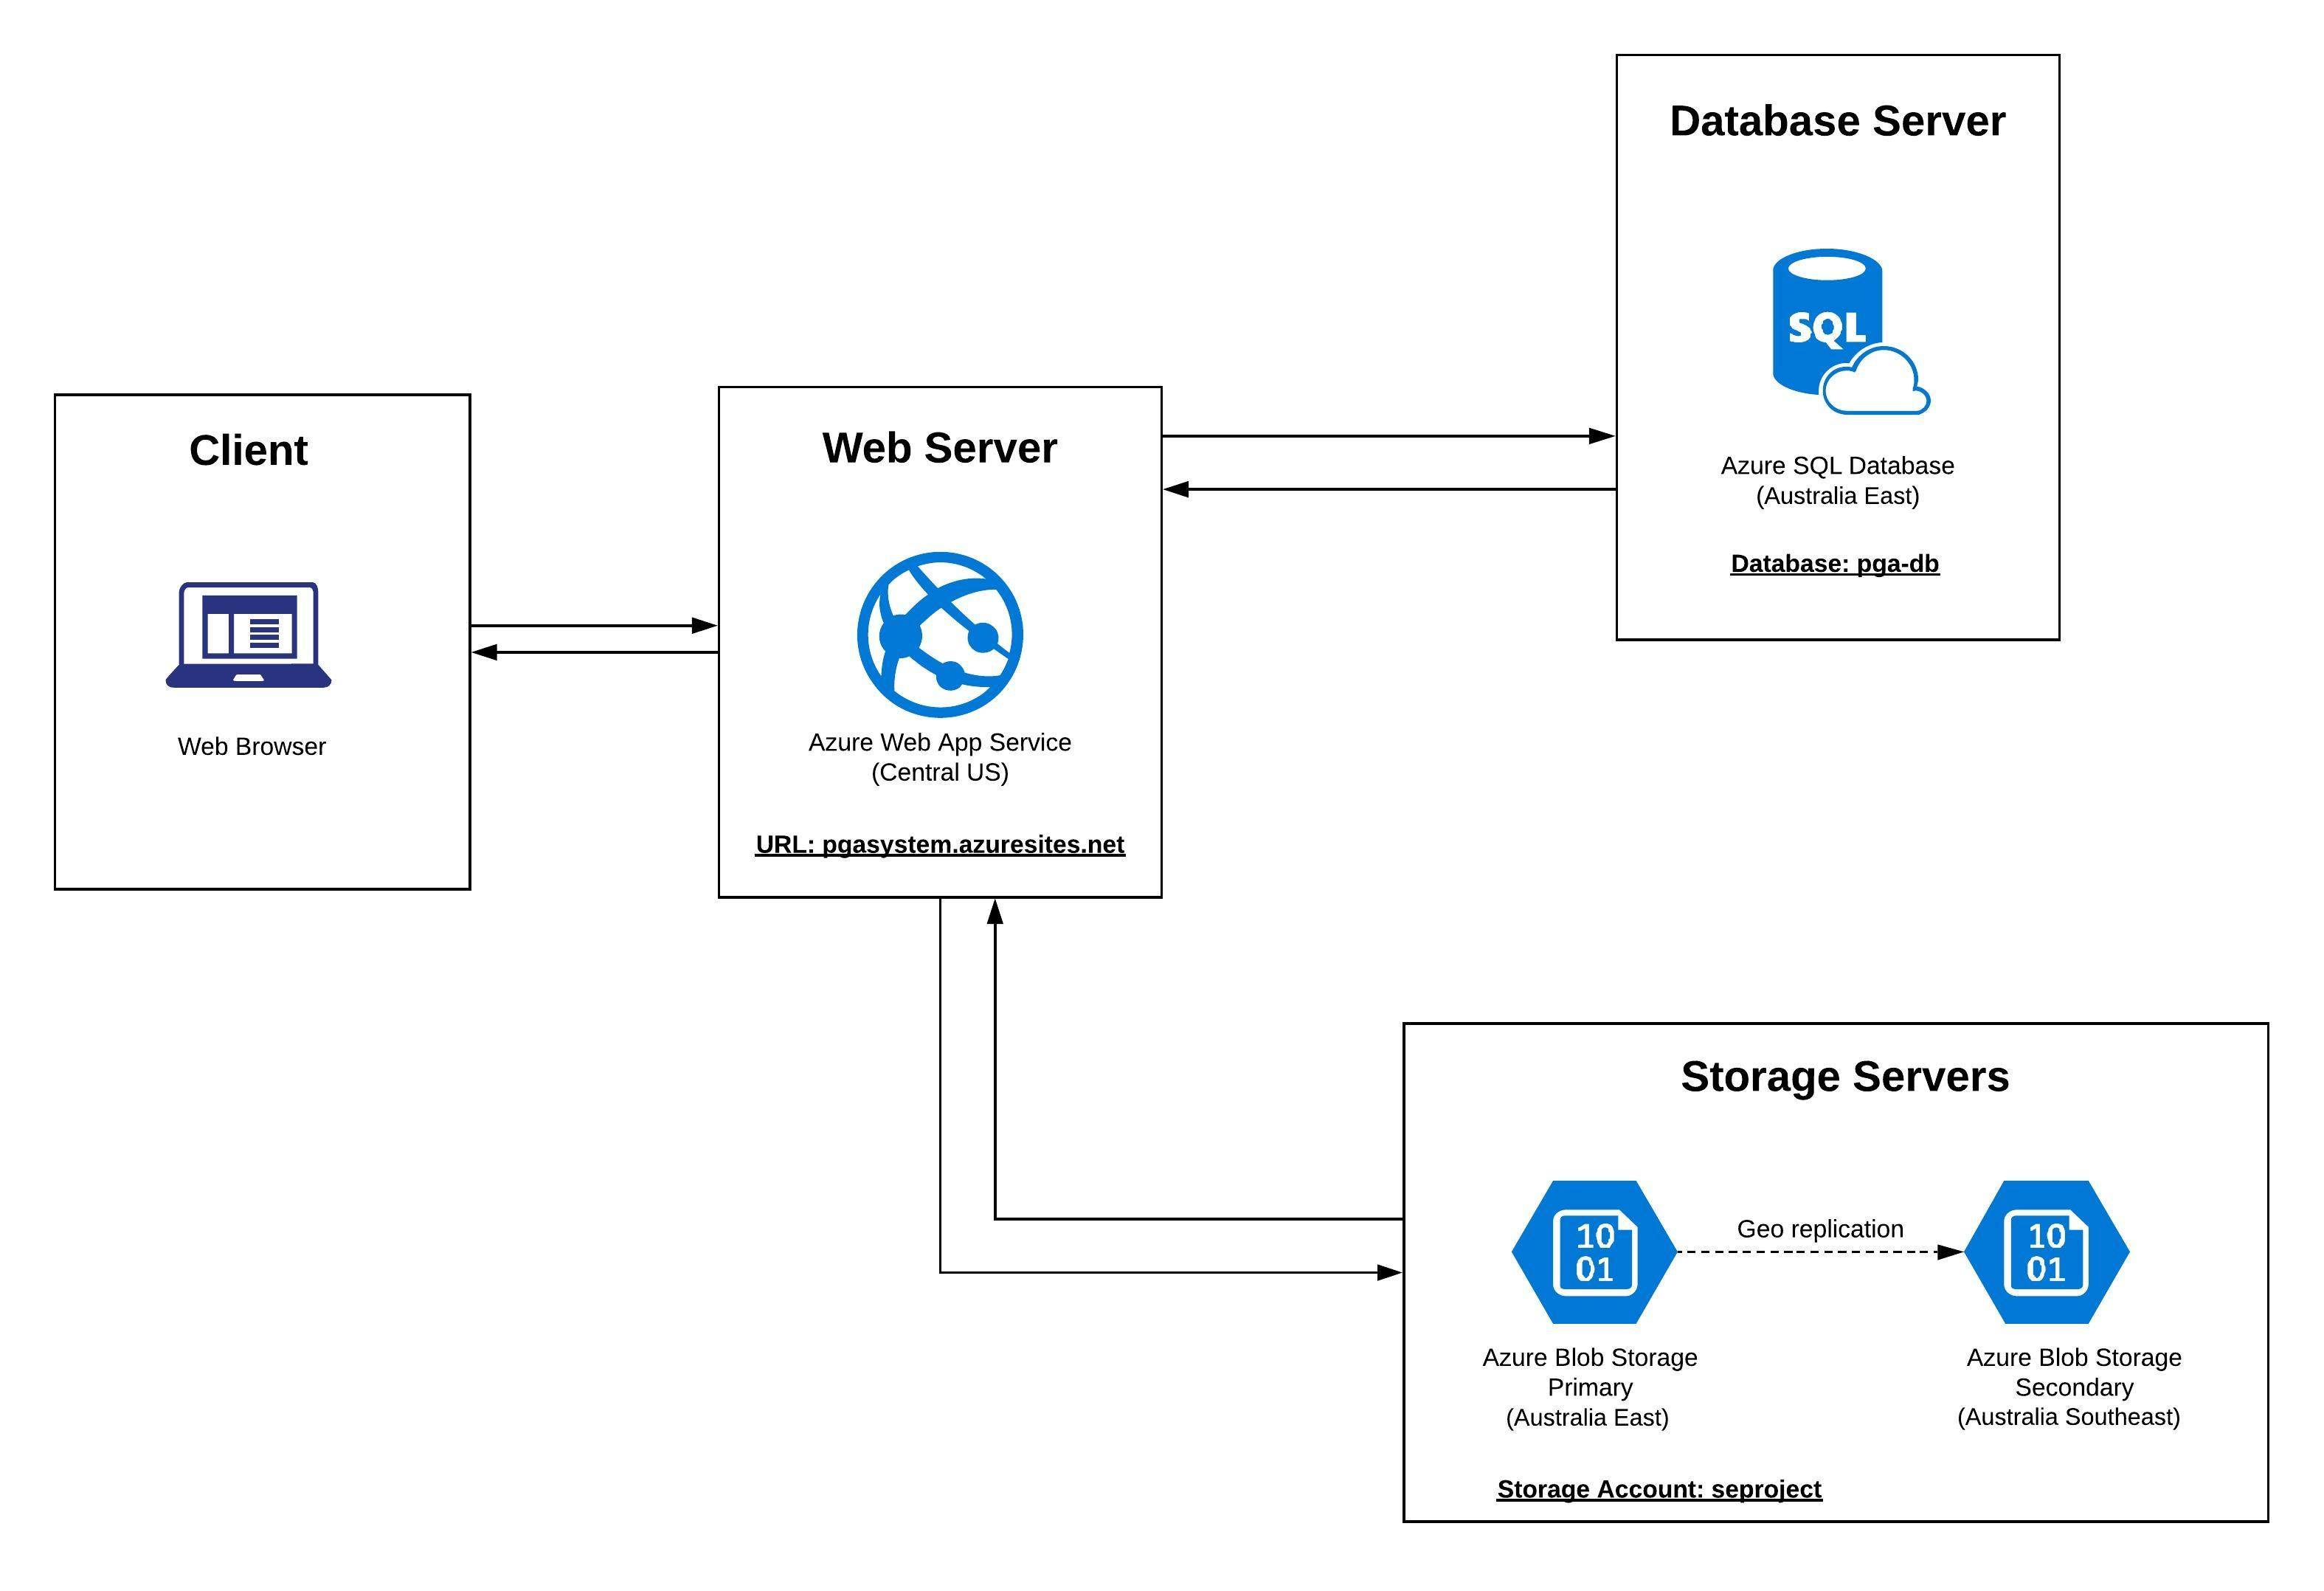
\includegraphics[width=\textwidth, height=\textheight, keepaspectratio]{Diagrams/HardwareArchitecture}}
	\caption{Hardware Architecture Diagram}
\end{figure}

architecture diagram, class view
\subsubsection{Overview}
\subsection{Process View}
\begin{figure}[H]
	\frame{\includegraphics[width=\textwidth, height=\textheight, keepaspectratio]{"Diagrams/ActivityDiagramCreateApplication"}}
	\caption{Activity Diagram for the Create Application Use Case}
\end{figure}
\begin{figure}[H]
	\frame{\includegraphics[width=\textwidth, height=\textheight, keepaspectratio]{"Diagrams/ActivityDiagramUpdateApplication"}}
	\caption{Activity Diagram for the Update Application Use Case}
\end{figure}
\subsection{Component View}
This section describes the User Interface for each user:

\subsubsection{Common User Screens}
\begin{figure}[H]
	\frame{\includegraphics[width=\textwidth, height=\textheight, keepaspectratio]{"Diagrams/Loginscreen"}}
	\caption{The Login Page}
\end{figure}
\subsubsection{Post Graduate Officer}
\begin{figure}[H]
	\frame{\includegraphics[width=\textwidth, height=\textheight, keepaspectratio]{"Diagrams/PGOHomePage"}}
	\caption{
		The PGO Logs in and lands on this screen.}
\end{figure}
\begin{figure}[H]
	\frame{\includegraphics[width=\textwidth, height=\textheight, keepaspectratio]{"Diagrams/CreateApplication"}}
	\caption{
		The PGO lands here when they click Create Application.}
\end{figure}


\begin{figure}[H]
	\frame{\includegraphics[width=\textwidth, height=\textheight, keepaspectratio]{"Diagrams/PGOViewApplications"}}
	\caption{The PGO lands here when they click Pending Applications from the home page. Here a list of applications with pending decisions, from either a Supervisor or the PGC, is displayed.}
\end{figure}
\begin{figure}[H]
	\frame{\includegraphics[width=\textwidth, height=\textheight, keepaspectratio]{"Diagrams/PGOViewApplication"}}
	\caption{Once the PGO selects an application to view, this screen is displayed. It displays applicant and application information as well as a file viewer.}
\end{figure}
\begin{figure}[H]
	\frame{\includegraphics[width=\textwidth, height=\textheight, keepaspectratio]{"Diagrams/PGOCompletedApplications"}}
	\caption{This page displays applications where the PGC has made a final decision.}
\end{figure}

\subsubsection{Supervisor}
\begin{figure}[H]
	\frame{\includegraphics[width=\textwidth, height=\textheight, keepaspectratio]{"Diagrams/SupervisorHomePage"}}
	\caption{The Landing Page for a Supervisor}
\end{figure}

\begin{figure}[H]
	\frame{\includegraphics[width=\textwidth, height=\textheight, keepaspectratio]{"Diagrams/SupervisorViewApplications"}}
	\caption{The Supervisor can see all pending applications that need their decision.}
\end{figure}
\begin{figure}[H]
	\frame{\includegraphics[width=\textwidth, height=\textheight, keepaspectratio]{"Diagrams/SupervisorViewApplication"}}
	\caption{The view application page for the Supervisor. It displays applicant and application information, a file viewer and a decision picker.}
\end{figure}
\subsubsection{Post Graduate Coordinator}
\begin{figure}[H]
	\frame{\includegraphics[width=\textwidth, height=\textheight, keepaspectratio]{"Diagrams/PGCHomePage"}}
	\caption{The Landing Page for the PGC}
\end{figure}

\begin{figure}[H]
	\frame{\includegraphics[width=\textwidth, height=\textheight, keepaspectratio]{"Diagrams/PGCViewApplications"}}
	\caption{The PGC can see all pending applications that have been accepted by a Supervisor that need final approval.}
\end{figure}
\begin{figure}[H]
	\frame{\includegraphics[width=\textwidth, height=\textheight, keepaspectratio]{"Diagrams/PGCViewApplication"}}
	\caption{The view application page for the PGC. It displays applicant and application information, a file viewer and a decision picker.}
\end{figure}

\subsection{Database View}
This section contains the Entity-Relationship Diagram for the System Database:
\begin{figure}[H]
	\frame{\includegraphics[width=\textwidth, height=\textheight, keepaspectratio]{"Diagrams/StressTestEssentials"}}
	\caption{Test Details}
\end{figure}


\section{Performance}
A stress test was conducted on the system. The Microsoft Azure performance testing framework was used. 
\subsection{Test Details and Results} The test details and results are as follows:
\begin{figure}[H]
	\frame{\includegraphics[width=\textwidth, height=\textheight, keepaspectratio]{"Diagrams/StressTestEssentials"}}
	\caption{Test Details}
\end{figure}

\begin{figure}[H]
	\frame{\includegraphics[width=\textwidth, height=\textheight, keepaspectratio]{"Diagrams/StressTestTemporalPlot"}}
	\caption{Temporal Plot of Average response time, the user load and the requests per second.}
\end{figure}
\begin{figure}[H]
	\frame{\includegraphics[width=\textwidth, height=\textheight, keepaspectratio]{"Diagrams/StressTestRequests"}}
	\caption{Test Results with 100\% request success.}
\end{figure}
\section{Quality}
This sections describes system quality concerns for future development on the system:
\begin{itemize}
	\item Use bundling and minifying of static css/js files to improve performance, see microsoft docs.
	\item Use caution when storing binary data in relational databases, as it can adversely impact performance.
	\item Using base64 string from byte array impacts page load times severely (5-10 second load time on a 214kb file). 
	
\end{itemize}


\end{document}

